\subsection{Observer Pattern}


\subsubsection*{Problembeschreibung}

Häufig müssen verschiedene Komponenten eines Systems synchron gehalten werden. Gleichzeitig soll aber auch eine enge Kopplung dieser Komponenten vermieden werden. Es wird eine $1$:$n$-Beziehung zwischen den Objekten benötigt, wobei $n$ Objekte von einem Objekt abhängen. Wenn das eine Objekt seinen Zustand ändert, so sollen alle abhängigen Objekte benachrichtigt werden, sodass auch sie ihren Zustand aktualisieren können. Ein naiver Lösungsansatz wäre, jedem abhängigen Objekt eine Referenz auf das Objekt zu geben, von welchem es abhängt. Die Objekte könnten dann in regelmäßigen Abständen prüfen, ob eine Zustandsänderung stattgefunden hat (\emph{Polling}). Dieser Ansatz weist jedoch nicht nur eine hohe Kopplung auf, er ist auch wenig performant. Auch wenn keine Zustandsänderung stattgefunden hat, wird auf diese geprüft. Der Aufwand für diese Prüfung steigt dabei linear mit der Anzahl der beteiligten Objekte.

Das \emph{Observer-Pattern} kann Anwendung finden, wenn es zwei voneinander getrennte Konzepte gibt und eines von dem anderen abhängig ist. Die Abhängigkeit muss modelliert werden können, ohne die Objekte stark zu koppeln. Weiterhin soll es möglich sein, die Anzahl der abhängigen Objekte variablen zu halten. \cite{gamma_design_1995}

\subsubsection*{Lösung}

Das Observer-Pattern besteht aus einem Sender (\code{Publisher}) und mehreren Empfängern (\code{ConcreteSubscriber}). Die Empfänger implementieren die Empfänger-Schnittstelle (\code{Subscriber}), welches eine Methode \code{update} zur Aktualisierung des Zustandes bereitstellt. Der Sender hält eine Liste von Referenzen auf Empfänger und verfügt über die Methoden \code{subscribe} und \code{unsubscribe}, welche es ermöglichen, der Liste Empfänger hinzuzufügen, oder sie zu entfernen (siehe Abbildung \ref{fig:observer-class}).

\begin{figure}[H]
	\centering
	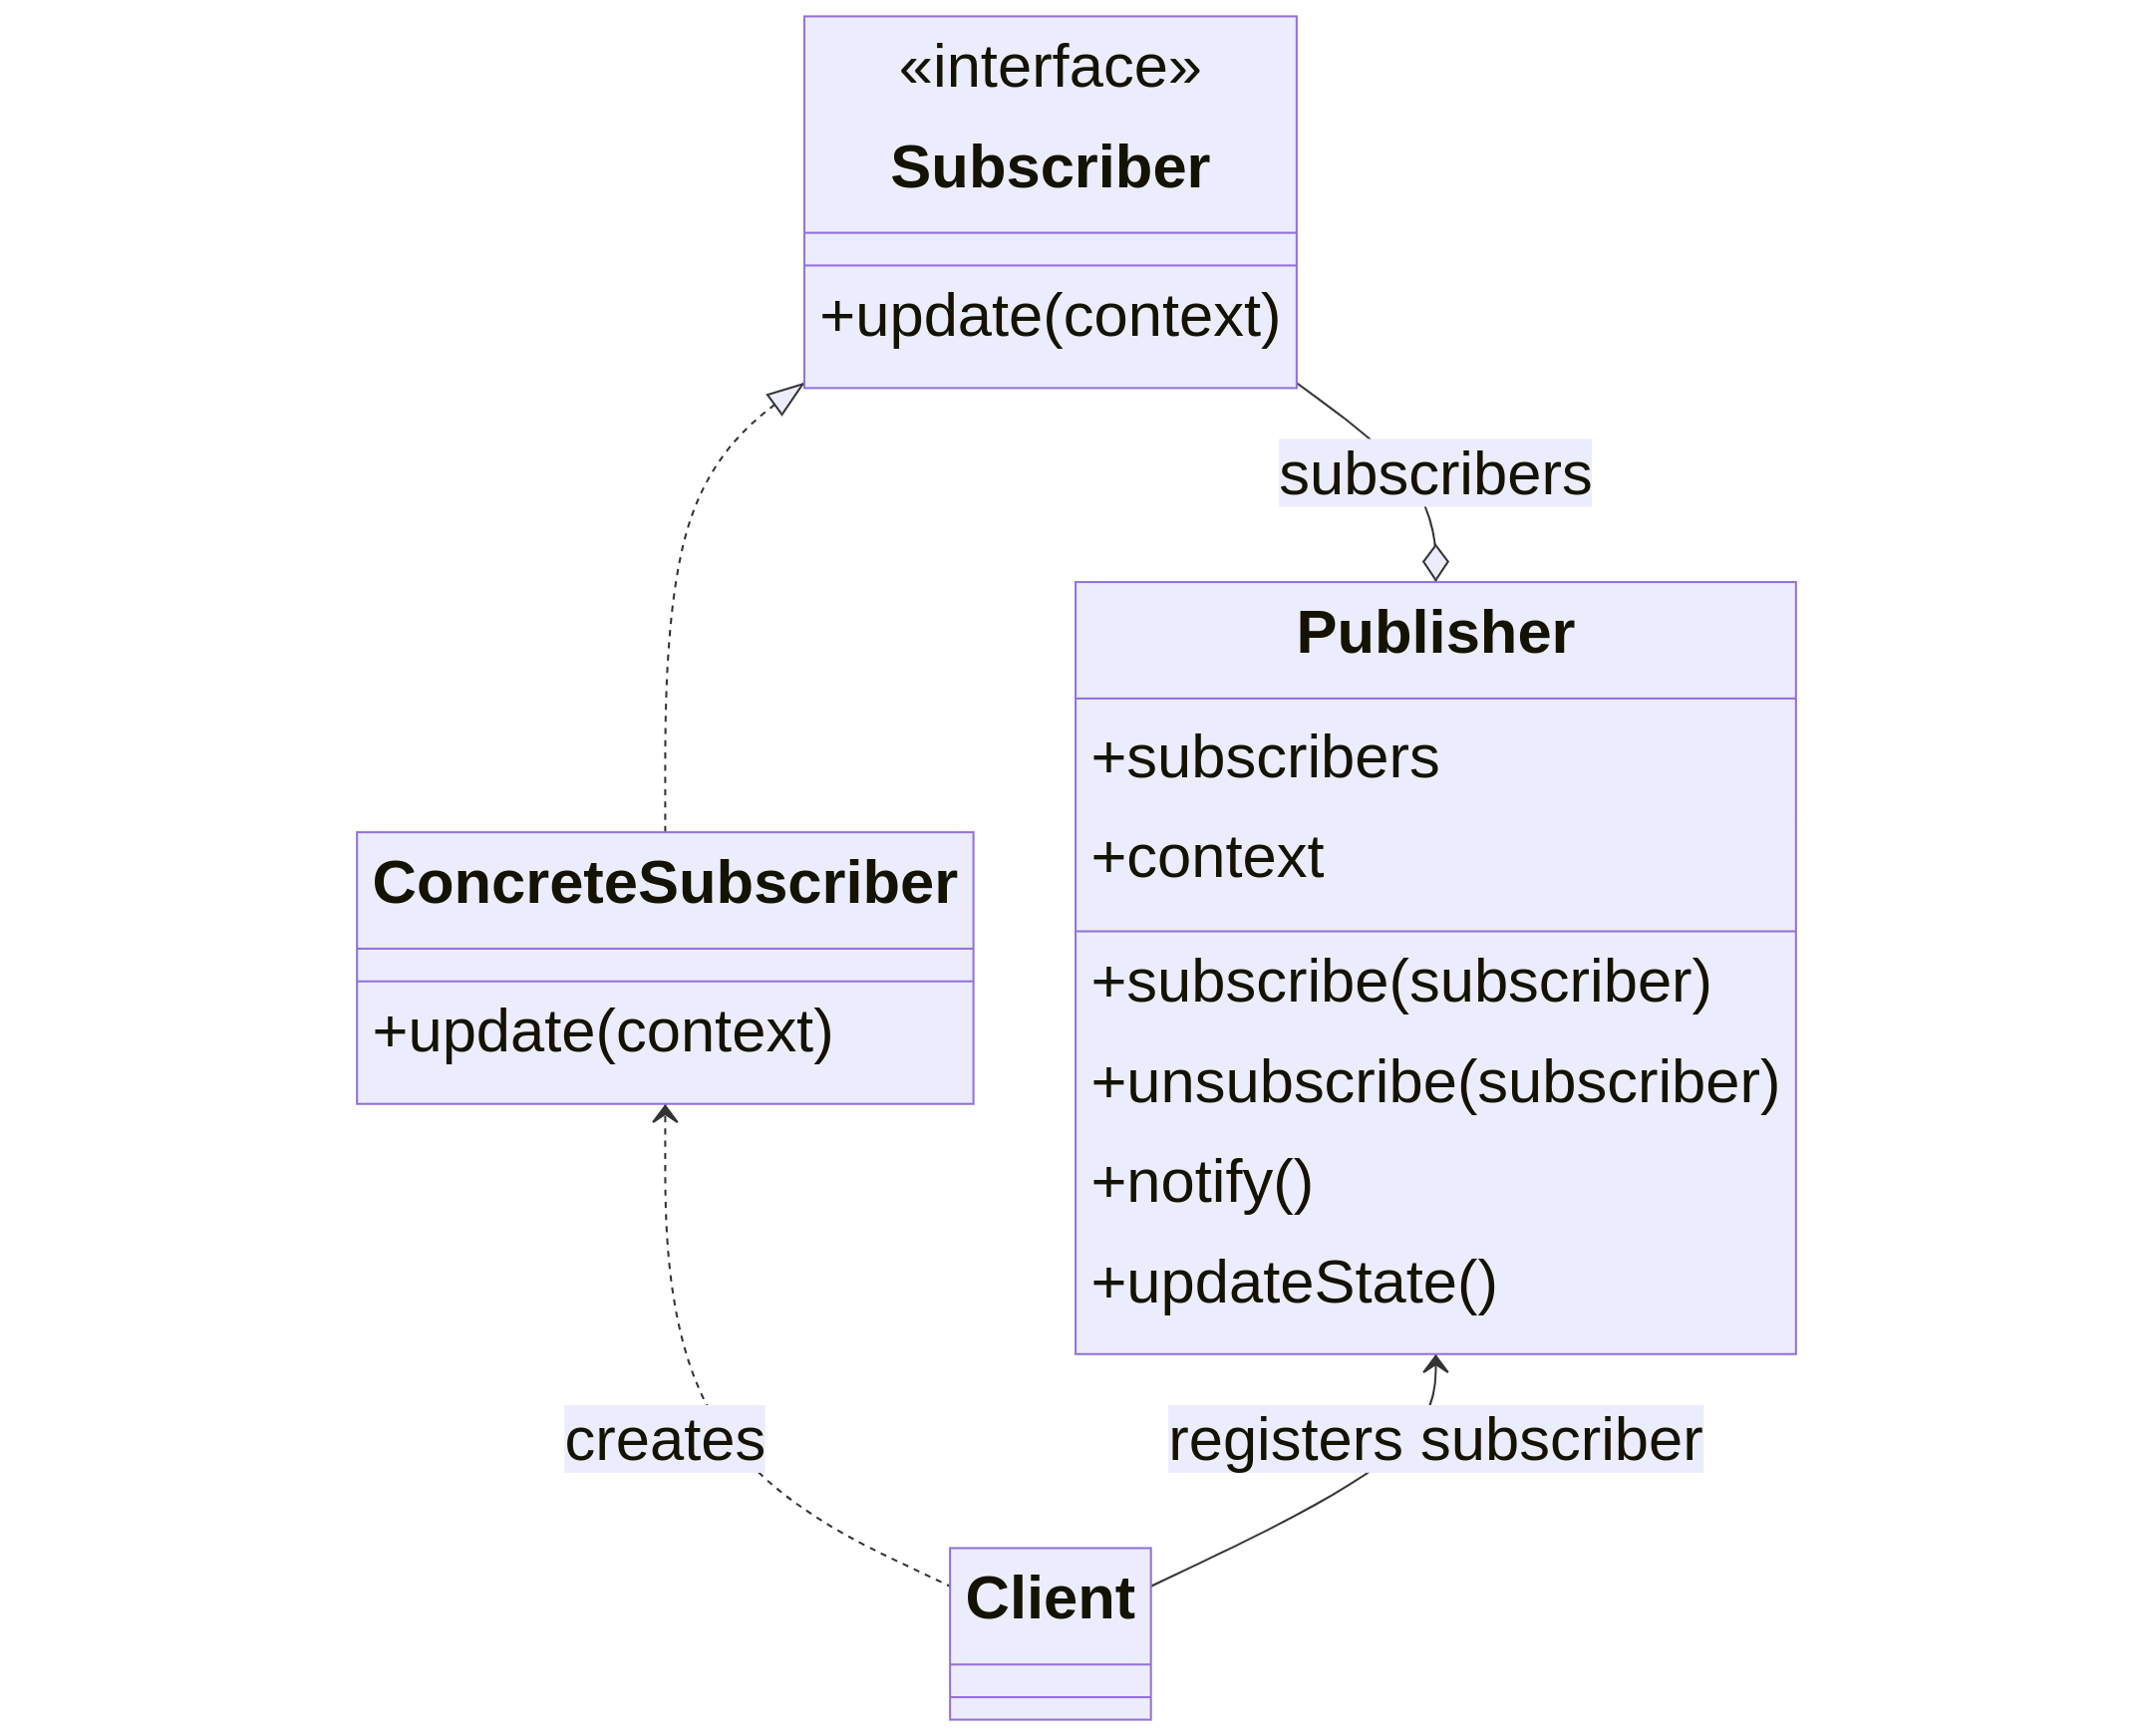
\includegraphics[width=0.95\linewidth]{images/patterns/observer-class.png}
	\caption{Klassendiagramm des Observer-Patterns \cite{skobeleva_observer_2023}}
	\label{fig:observer-class}
\end{figure}

Abbildung \ref{fig:observer-seq} zeigt, dass der Anwender (\code{Client})\footref{ftn:client} den Zustand des Sender durch Senden von \code{updateSate} verändern kann (1). Der Sender sendet sich draufhin selbst \code{notify} (2) und beginnt über seine Liste von Empfängern zu iterieren. Jedem Empfänger sendet er dann \code{update} (3, 5) und übergibt den notwendigen Kontext, sodass der Empfänger seinen Zustand entsprechend aktualisieren kann.

\begin{figure}[H]
	\centering
	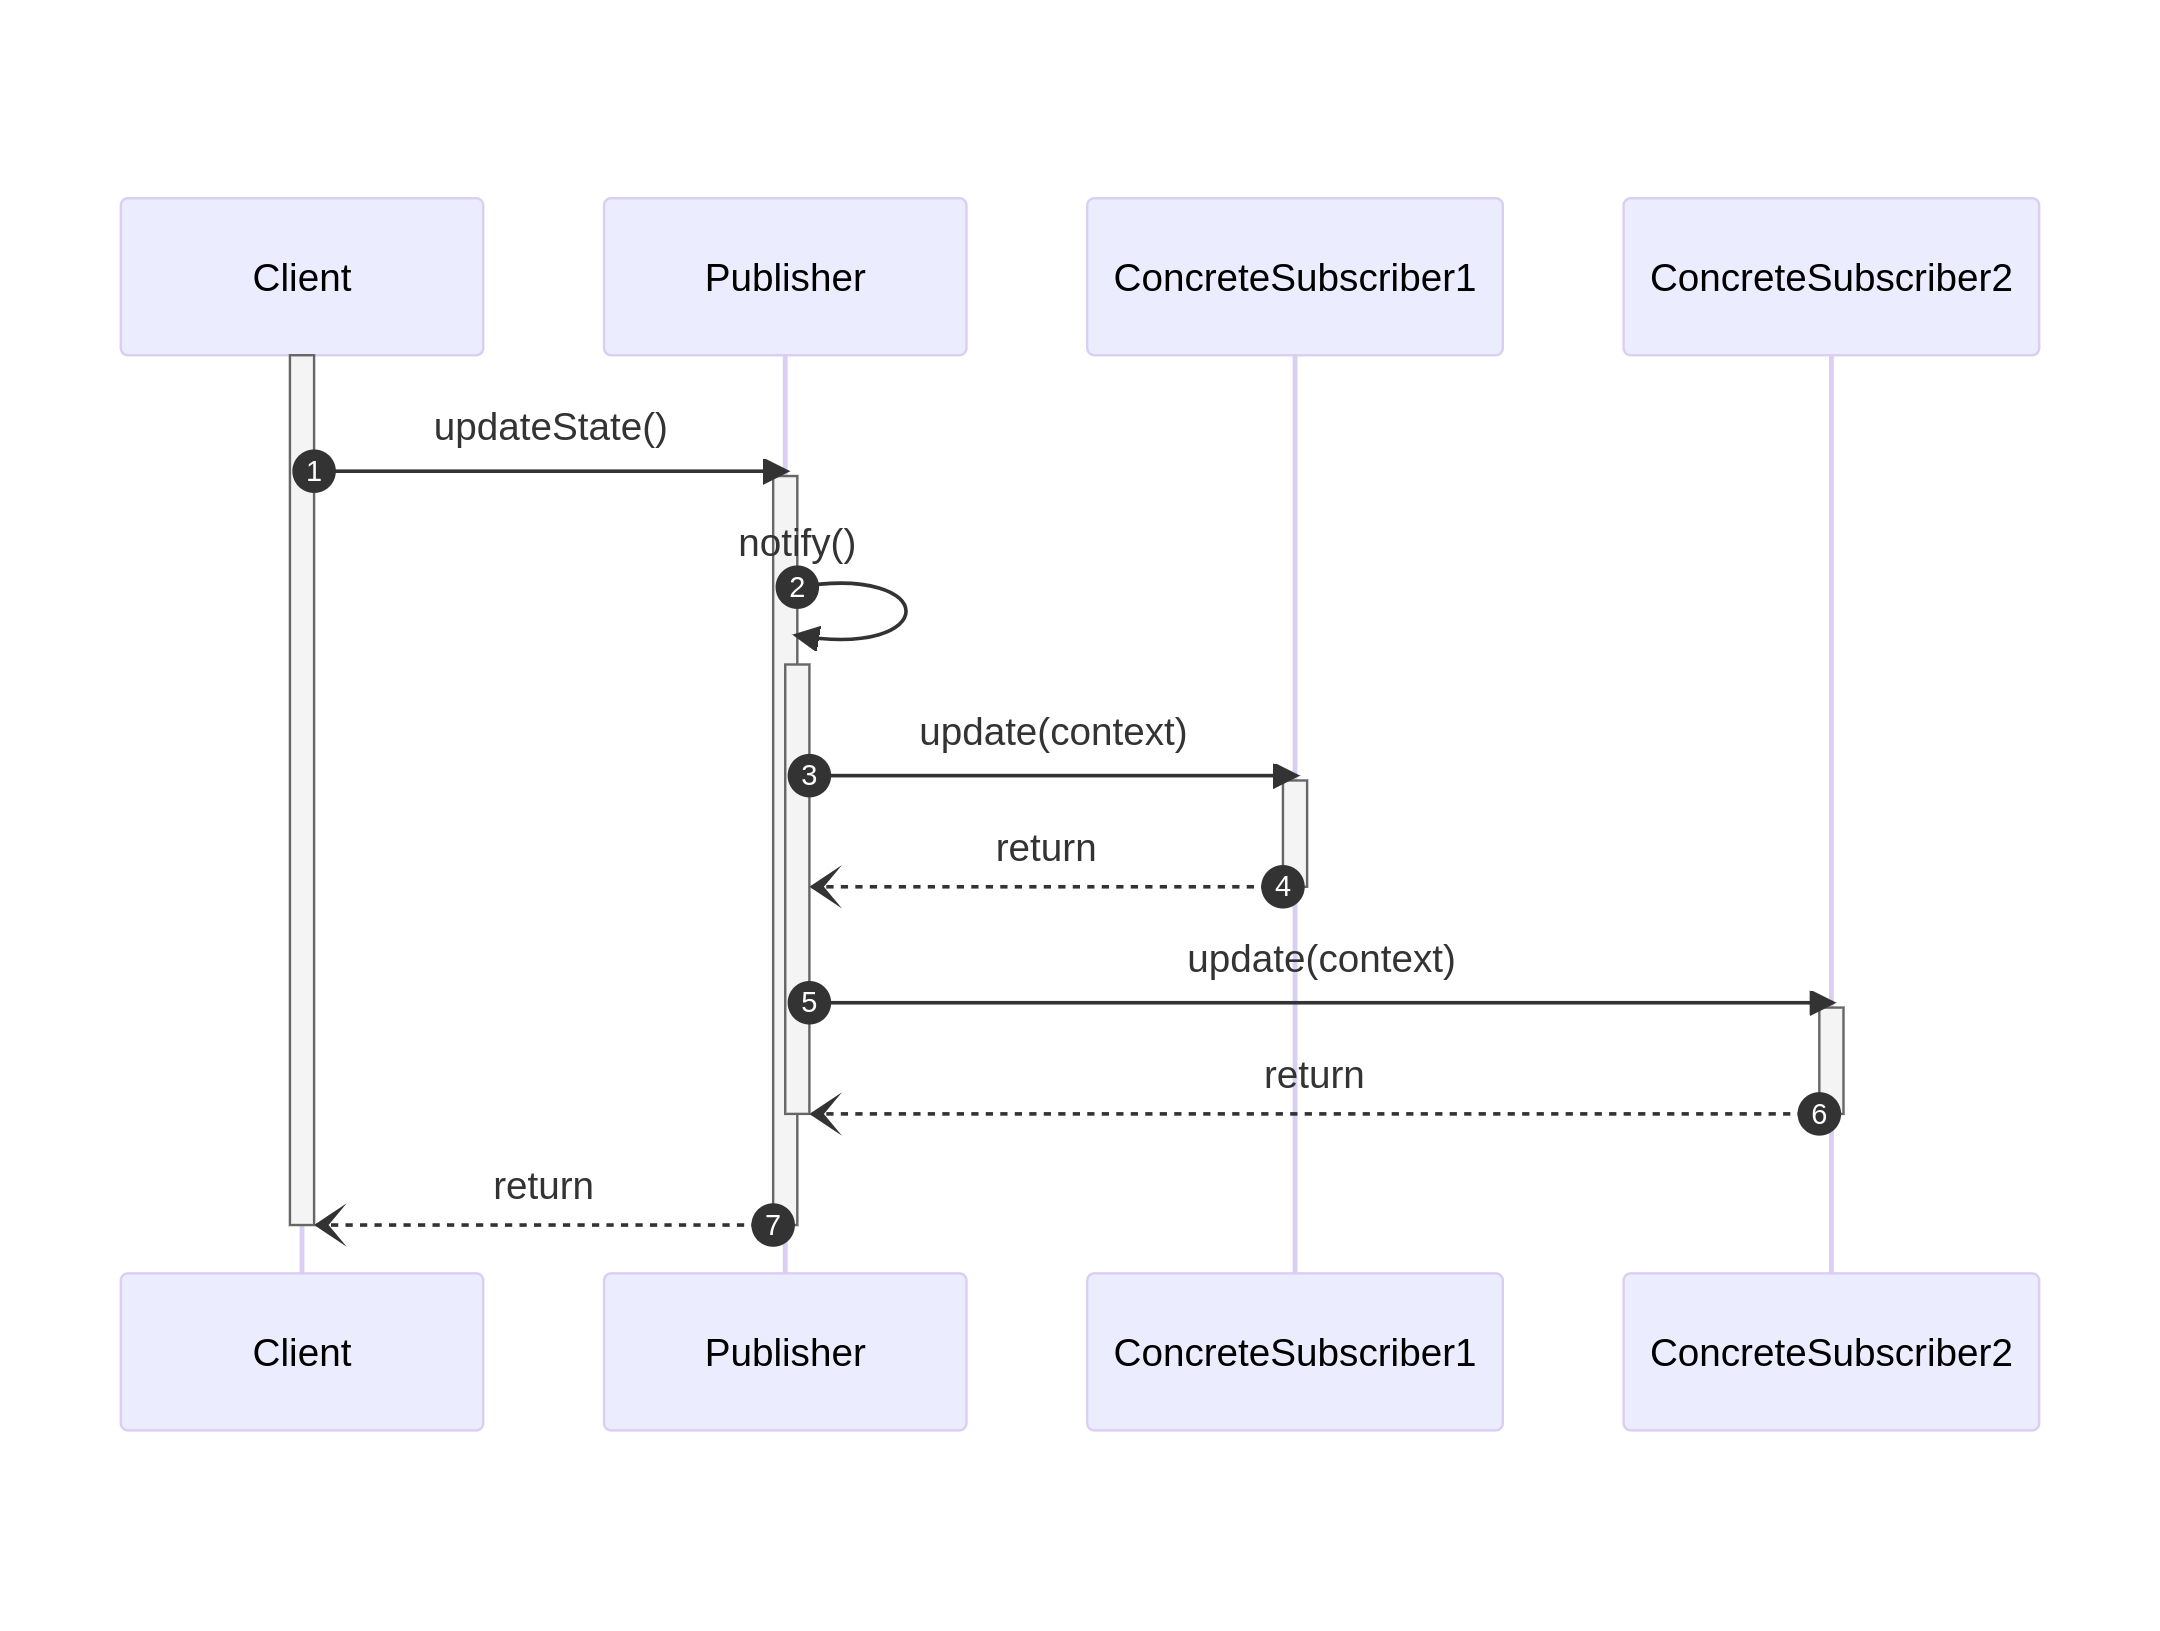
\includegraphics[width=0.95\linewidth]{images/patterns/observer-seq.png}
	\caption{Sequenzdiagramm des Observer-Patterns \cite{skobeleva_observer_2023}}
	\label{fig:observer-seq}
\end{figure}

Quelltext \ref{code:observer-code} veranschaulicht die Benachrichtigung aller Empfänger. In \code{notify} wird an jeden im Sender referenzierten Empfänger \code{update} gesendet. Dabei wird der Kontext des Senders an jeden Empfänger übergeben.

\lstset{language=python}
\begin{lstlisting}[caption={Quelltext der Methode \code{notify} des Publishers, welche über alle Empfänger iteriert und diese benachrichtigt.}, label=code:observer-code]
class Publisher
	def notify(self):
        for subscriber in self.subscribers:
            subscriber.update(self.context)
\end{lstlisting}


\subsubsection*{Konsequenzen}

Durch Separation von Sender und Empfänger und durch die Abstraktion der Empfänger-Schnittstelle wird eine lose Kopplung der beiden erreicht. Diese lose Kopplung ermöglicht es, sowohl den Sender, als auch die Empfänger beliebig auszutauschen. Weiterhin können sich der Sender und die Empfänger auf unterschiedlichen Abstraktionsniveaus befinden. Ein Sender auf einem niedrigen Level kann einen Empfänger auf einem hohen Level benachrichtigen. Wären Empfänger und Sender nicht getrennt, so wäre dafür ein Objekt notwendig, welches mehrere Abrstraktionsebenen umfasst, wodurch die Trennung der Abstraktionsschichten beeinträchtigen würde. Ein weiterer Vorteil ist die dynamische Anzahl der Empfänger, mit denen ein Sender interagieren kann. So kann der Anwender über den Sender eine beliebige Zahl an Empfängern erreichen.

Ein Nachteil des Observer-Patterns ist, dass der Sender stets alle seine Empfänger benachrichtigt. Es kann vorkommen, dass nur eine Teilmenge der Empfänger die Benachrichtigung benötigt, was in unnötigen Methodenaufrufen resultiert. \cite{gamma_design_1995}